\section{反演器}
\markboth{69. 反演器}{69. 反演器}

\noindent
\begin{minipage}[t]{0.53\textwidth}
  \vspace{0pt}
  \hspace*{2em}画一条曲线的反演图形，通常是一个点一个点地求出若干点的反演对应点，再连成曲线。如果有图 69.1 所示的反演器的帮助，画图就简便多了。这种反演器由六根杆连接而成，在连接点 $O$、$A$、$B$、$C$、$D$ 都可以自由转动，$OC$ 和 $OD$ 两根杆的长度相等，其余四根杆的长度彼此相等。在 $B$ 点处装了一支笔，让 $O$ 点在纸上固定不动，$A$ 点沿着已知曲线移动，$B$ 处的笔就会画出已知曲线的反演图形来。
\end{minipage}\hfill
\begin{minipage}[t]{0.44\textwidth}
  \vspace{2pt}
  \centering
  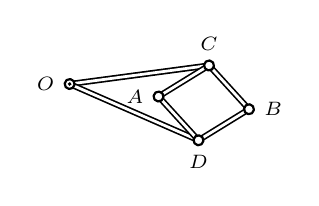
\begin{tikzpicture}[scale=1.0, rotate=-8, line cap=round, line join=round]
    \coordinate (O) at (0,0);
    \coordinate (C) at (1.72, 0.48);
    \coordinate (D) at (1.72, -0.48);
    \coordinate (A) at (1.14, 0);
    \coordinate (B) at (2.30, 0);

    % 六根连杆（双线杆件风格）
    \foreach \p/\q in {O/C, O/D, A/C, A/D, B/C, B/D} {
      \draw[line width=2.2pt] (\p) -- (\q);
      \draw[line width=1.0pt, white] (\p) -- (\q);
    }

    % 铰链圆点
    \foreach \p in {O, A, B, C, D} {
      \fill[white] (\p) circle (1.8pt);
      \draw[thick] (\p) circle (1.8pt);
    }
    \fill (O) circle (0.7pt);

    \node[left=2pt, font=\scriptsize] at (O) {$O$};
    \node[left=2pt, font=\scriptsize] at (A) {$A$};
    \node[right=2pt, font=\scriptsize] at (B) {$B$};
    \node[above=2pt, font=\scriptsize] at (C) {$C$};
    \node[below=2pt, font=\scriptsize] at (D) {$D$};
  \end{tikzpicture}
  \captionof*{figure}{图\ 69.1}
\end{minipage}

为了说明上述反演器的原理，我们注意

\noindent
\begin{minipage}[t]{0.44\textwidth}
  \vspace{2pt}
  \centering
  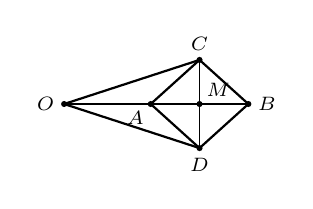
\begin{tikzpicture}[scale=1.0, line cap=round, line join=round]
    \coordinate (O) at (0,0);
    \coordinate (C) at (1.72, 0.56);
    \coordinate (D) at (1.72, -0.56);
    \coordinate (M) at (1.72, 0);
    \coordinate (A) at (1.10, 0);
    \coordinate (B) at (2.34, 0);

    \draw[thick] (O) -- (C) -- (B) -- (D) -- cycle;
    \draw[thick] (A) -- (C);
    \draw[thick] (A) -- (D);
    \draw (O) -- (B);
    \draw (C) -- (D);

    \fill (O) circle (1.1pt) node[left, font=\scriptsize] {$O$};
    \fill (A) circle (1.1pt) node[below left=-1pt, font=\scriptsize] {$A$};
    \fill (B) circle (1.1pt) node[right, font=\scriptsize] {$B$};
    \fill (C) circle (1.1pt) node[above, font=\scriptsize] {$C$};
    \fill (D) circle (1.1pt) node[below, font=\scriptsize] {$D$};
    \fill (M) circle (1.1pt) node[above right=-1pt, font=\scriptsize] {$M$};
  \end{tikzpicture}
  \captionof*{figure}{图\ 69.2}
\end{minipage}
\hfill
\begin{minipage}[t]{0.53\textwidth}
  \vspace{0pt}
  \begin{gather*}
    OC = OD,\quad AC = AD, \\
    BC = BD,
  \end{gather*}
  因而 $O$、$A$、$B$ 都在线段 $CD$ 的垂直平分线上，即三点 $O$、$A$、$B$ 在一直线上。如图 69.2，设 $CD$ 与 $AB$ 的交点为 $M$。
\end{minipage}

\medskip
\noindent
因为 $ACBD$ 是菱形，所以 $AM=MB$。由此得到
\begin{align*}
  OA\cdot OB &= (OM - AM)(OM + MB) \\
             &= OM^2 - MB^2.
\end{align*}
另一方面，
\begin{align*}
  OM^2 - MB^2 &= (OM^2 + MC^2) - (MB^2 + MC^2) \\
              &= OC^2 - BC^2,
\end{align*}
而 $OC$ 和 $BC$ 都是定长，所以
\[
  OA\cdot OB = OC^2 - BC^2 = \text{定值}.
\]
这样就证明了，只要保持 $O$ 点的位置不变，不论 $A$ 点移动到什么位置，$B$ 都是 $A$ 的反点，反演极为 $O$，反演幂为 $OC^2 - BC^2$。所以当 $A$ 沿着一条曲线移动时，$B$ 就画出这条曲线的反演图形。
